\documentclass[11pt,letterpaper]{article}
% Shared macros for QVC arXiv v4 (main + TQGL supplement)
% Locked Option A* numbers (fat torus, Tier-C form, frozen-cavity bridge).

\usepackage[utf8]{inputenc}
\usepackage[T1]{fontenc}
\usepackage{amsmath,amssymb,amsthm,mathtools}
\usepackage{graphicx}
\usepackage{caption}
\usepackage{subcaption}
\usepackage{hyperref}
\usepackage{geometry}
\usepackage{float}
\usepackage[section]{placeins}   % FloatBarrier at every \section
\usepackage{tikz}
\usetikzlibrary{arrows.meta,decorations.pathmorphing,positioning,shapes.geometric,calc,3d,fit,backgrounds}
\usepackage{tikz-3dplot}
\usepackage{pgfplots}
\pgfplotsset{compat=1.18}
\usepackage{booktabs}
\usepackage{bm}
\usepackage{xcolor}
\usepackage{enumitem}
\usepackage{array}
\usepackage{multirow}
\usepackage[expansion=false]{microtype}

\geometry{margin=1in}

% Okabe--Ito (colorblind-safe)
\definecolor{oiOrange}{HTML}{E69F00}
\definecolor{oiSky}{HTML}{56B4E9}
\definecolor{oiGreen}{HTML}{009E73}
\definecolor{oiYellow}{HTML}{F0E442}
\definecolor{oiBlue}{HTML}{0072B2}
\definecolor{oiVerm}{HTML}{D55E00}
\definecolor{oiPurple}{HTML}{CC79A7}

\hypersetup{
  colorlinks=true,
  linkcolor=oiBlue,
  citecolor=oiVerm,
  urlcolor=oiBlue,
  pdfauthor={Mineral Hoiland},
  pdftitle={Quantum Vacuum Catalyzation in Topological Excitonic Systems}
}

\newtheorem{theorem}{Theorem}[section]
\newtheorem{lemma}[theorem]{Lemma}
\newtheorem{proposition}[theorem]{Proposition}
\newtheorem{corollary}[theorem]{Corollary}
\newtheorem{definition}[theorem]{Definition}
\newtheorem{remark}[theorem]{Remark}
\newtheorem{hypothesis}{Hypothesis}

\newcommand{\TEVC}{\textsc{TEVC}}
\newcommand{\QVC}{\textsc{QVC}}
\newcommand{\TQGL}{\textsc{TQGL}}
\newcommand{\BKT}{\textsc{BKT}}
\newcommand{\MATBG}{\textsc{MATBG}}
\newcommand{\DCE}{\textsc{DCE}}
\newcommand{\TDVT}{\textsc{TDVT}}
\newcommand{\GPE}{\textsc{GPE}}

\newcommand{\abs}[1]{\left|#1\right|}
\newcommand{\norm}[1]{\left\|#1\right\|}
\newcommand{\dd}[1]{\,\mathrm{d}#1}

% Locked Option A* (fat torus, Tier-C form, frozen-cavity bridge)
\newcommand{\Evac}{0.1287\,\mathrm{meV}}
\newcommand{\Flock}{0.58068}
\newcommand{\elllock}{-2.7958}
\newcommand{\ellcorr}{-2.791}
\newcommand{\alphac}{0.1818}
\newcommand{\Deltac}{0.109\,\mathrm{meV}}
\newcommand{\Deltaex}{0.600\,\mathrm{meV}}
\newcommand{\lfold}{0.8475}
\newcommand{\lstar}{0.7628}
\newcommand{\Deltastar}{0.2324\,\mathrm{meV}}
\newcommand{\hbarcs}{0.07\,\mathrm{meV\cdot\mu m}}
\newcommand{\etaret}{0.137} % a_H evaluation; unique-lock pair is \etaretaH and \etaretph
\newcommand{\etaretaH}{0.137}
\newcommand{\etaretph}{2}
\newcommand{\etaretalt}{3.1}
\newcommand{\xiph}{117\,\mathrm{nm}}
\newcommand{\xialt}{181\,\mathrm{nm}}
\newcommand{\aHlock}{8\,\mathrm{nm}}
\newcommand{\kappaGL}{3.84\times 10^{-5}\,\mathrm{meV\cdot\mu m}^{2}}
\newcommand{\alphaGL}{-0.600\,\mathrm{meV}}
\newcommand{\betaGL}{0.694\,\mathrm{meV}}
\newcommand{\nrefhopf}{0.864}
\newcommand{\alphastar}{0.1636}
\newcommand{\kappaSansatz}{2.46\times 10^{-9}\,\mathrm{meV\cdot\mu m}^{4}}
\newcommand{\Deltacat}{0.502\,\mathrm{meV}}
\newcommand{\gzerofold}{0.109\,\mathrm{meV}}
\newcommand{\pctcat}{16.4\%}
\newcommand{\pctcatfold}{18.2\%}
\newcommand{\hatbarrier}{30\%}
\newcommand{\RwsMatch}{2.18\,\mu\mathrm{m}}
\newcommand{\RwsAlt}{0.91\,\mu\mathrm{m}}
\newcommand{\dsigmaH}{3.87\times 10^{-6}\,\mathrm{S}}
\newcommand{\gzeroeff}{1.365\times 10^{-4}}
\newcommand{\relfroG}{0.0667}
\newcommand{\gzeroeffring}{5.472\times 10^{-4}}
\newcommand{\relfroGring}{0.1564}
\newcommand{\specGws}{\bigl(-1.568,-1.568,-1.162,-1.160,+5.458\bigr)\times 10^{-4}}
\newcommand{\specGring}{\bigl(-7.385,-7.247,-4.326,-2.930,+21.888\bigr)\times 10^{-4}}
\newcommand{\Deltataufive}{0.5720\,\mathrm{meV}}
\newcommand{\gonetaufive}{0.7102}
\newcommand{\Deltatautwenty}{0.6152\,\mathrm{meV}}
\newcommand{\gonetautwenty}{0.8351}
\newcommand{\Deltataufifty}{0.6248\,\mathrm{meV}}
\newcommand{\gonetaufifty}{0.8639}
\newcommand{\Deltanumonly}{0.5697\,\mathrm{meV}}
\newcommand{\gonumonly}{0.8806}
\newcommand{\Deltadephonly}{0.6309\,\mathrm{meV}}
\newcommand{\godephonly}{0.7031}
\newcommand{\Deltafrozencoherent}{0.6623\,\mathrm{meV}}
\newcommand{\gofrozencoherent}{0.1075}
\newcommand{\Deltafrozentaufive}{0.0872\,\mathrm{meV}}
\newcommand{\gofrozentaufive}{0.0102}
\newcommand{\Deltafrozentautwenty}{0.3920\,\mathrm{meV}}
\newcommand{\gofrozentautwenty}{0.0812}
\newcommand{\Deltafrozentaufifty}{0.4761\,\mathrm{meV}}
\newcommand{\gofrozentaufifty}{0.0032}
\newcommand{\gzeroscaled}{0.0527\,\mathrm{meV}}
\newcommand{\lamcat}{0.410}
\newcommand{\redstar}{61.3\%}
\newcommand{\redmax}{81.8\%}
% Coupled GPE / DCE suite (live gap from psi)
\newcommand{\Deltaliveone}{0.6305\,\mathrm{meV}}
\newcommand{\goneps}{0.8832}
\newcommand{\AoneAc}{0.9811}
\newcommand{\AresAc}{0.9117}
\newcommand{\AdetAc}{0.8800}
\newcommand{\Deltassres}{0.2240\,\mathrm{meV}}
\newcommand{\Deltassdet}{0.2461\,\mathrm{meV}}
\newcommand{\gzerostar}{0.0982\,\mathrm{meV}}
\newcommand{\Epair}{0.1963\,\mathrm{meV}}
\newcommand{\Tstar}{118.7\,\mathrm{mK}}
\newcommand{\BerryR}{0.908}
\newcommand{\AcSch}{8.571\,\mu\mathrm{m}^{-1}}
\newcommand{\Acfold}{1.5582\,\mu\mathrm{m}^{-1}}
\newcommand{\gzerohess}{0.0185\,\mathrm{meV}}
\newcommand{\taudark}{662\,\mathrm{ps}}
\newcommand{\taubright}{10.1\,\mathrm{ps}}
\newcommand{\tauratio}{65}
\newcommand{\fluxerr}{3.8\times 10^{-4}}
\newcommand{\Kcanon}{0.407}
\newcommand{\ChernQWZ}{0.993}
\newcommand{\kgeomQWZ}{0.0430\,\mathrm{meV}}
\newcommand{\kgeomfloor}{0.0955\,\mathrm{meV}}
\newcommand{\kconvuv}{0.382\,\mathrm{meV}}
\newcommand{\kappauvtoy}{0.425\,\mathrm{meV}}
\newcommand{\etauv}{0.050}
\newcommand{\etauvsw}{0.053}
\newcommand{\QhopfSthree}{0.9998}
\newcommand{\attachrms}{3.8\times 10^{-16}}
\newcommand{\tlamoverU}{0.379}
\newcommand{\UoverWgap}{0.111}
\newcommand{\KuvTstar}{41.6}
\newcommand{\KfoldTstar}{5.44}
\newcommand{\tlammeV}{0.227\,\mathrm{meV}}
\newcommand{\Wmoire}{5.38\,\mathrm{meV}}
\newcommand{\massdriftcs}{8.3\times 10^{-6}}
\newcommand{\kappafoldtoy}{0.0556\,\mathrm{meV}}
\newcommand{\mstaroverme}{0.99}
\newcommand{\hwphaH}{8.75\,\mathrm{meV}}
\newcommand{\csBog}{1.06\times 10^{5}\,\mathrm{m/s}}
\newcommand{\cLA}{2.14\times 10^{4}\,\mathrm{m/s}}
\newcommand{\nuGPE}{0.290\,\mathrm{THz}}
\newcommand{\omegaGPEps}{1.82\,\mathrm{ps}^{-1}}
\newcommand{\nuStar}{0.112\,\mathrm{THz}}
\newcommand{\qstarLA}{0.0330\,\mathrm{nm}^{-1}}
\newcommand{\lamresLA}{190\,\mathrm{nm}}
\newcommand{\qoverKM}{0.102}
\newcommand{\lamresCS}{0.95\,\mu\mathrm{m}}
\newcommand{\Cvkmin}{0.430\,\mathrm{meV}}
\newcommand{\kappauvfloor}{0.477\,\mathrm{meV}}
\newcommand{\Kuvfloor}{46.7}
\newcommand{\Kfoldfloor}{10.57}
\newcommand{\Fmoire}{1.119}
\newcommand{\Fmoir}{\mathcal{F}_{\text{moir\'{e}}}}
\newcommand{\Ageom}{1.839\,\mu\mathrm{m}^{-1}}
\newcommand{\AgeomF}{2.058\,\mu\mathrm{m}^{-1}}
\newcommand{\lfoldF}{0.7573}
\newcommand{\lstarF}{0.6816}
\newcommand{\DeltaStarF}{0.2914\,\mathrm{meV}}
\newcommand{\GammaschHz}{5.30\times 10^{2}\,\mathrm{Hz}}
\newcommand{\schexp}{19.20}
\newcommand{\qIRpaper}{3.65\times 10^{3}\,\mu\mathrm{m}^{-1}}
\newcommand{\LambdaUV}{125\,\mu\mathrm{m}^{-1}}
\newcommand{\qgapIR}{8.57\,\mu\mathrm{m}^{-1}}

\graphicspath{{figures/}}

% Status tags (use sparingly in running text)
\newcommand{\statusproven}{\textup{\textsc{proven}}}
\newcommand{\statuscomputed}{\textup{\textsc{computed}}}
\newcommand{\statusworking}{\textup{\textsc{frozen working}}}
\newcommand{\statusprogram}{\textup{\textsc{program}}}
\newcommand{\statusconjecture}{\textup{\textsc{conjecture}}}
\newcommand{\statusansatz}{\textup{\textsc{ansatz}}}
\newcommand{\statusmatched}{\textup{\textsc{matched}}}
\newcommand{\statuslocked}{\textup{\textsc{locked}}}
\newcommand{\statusderived}{\textup{\textsc{derived here}}}
\newcommand{\statustruncated}{\textup{\textsc{truncated}}}
\newcommand{\statusdiag}{\textup{\textsc{diagnostic}}}


\title{\textbf{Supplemental Material: Truncated Topological Ginzburg--Landau Dynamics}\\
\large Truncated GPE, live gap, dynamical Casimir ODE, and $G_{ij}$\\
\large Companion to the QVC preprint}
\author{Mineral Hoiland\\
\textit{Independent Researcher}\\
\href{mailto:mineralhoilandphysics@gmail.com}{mineralhoilandphysics@gmail.com}\\
ORCID: \href{https://orcid.org/0009-0001-2696-644X}{0009-0001-2696-644X}}
\date{8 September 2026}

\begin{document}
\maketitle

\begin{abstract}
This supplement specifies the dynamical content of Quantum Vacuum Catalyzation (\QVC) that is \emph{actually} integrated, as distinct from the parent Topological Ginzburg--Landau (\TQGL) functional written in the companion preprint. The time stepper is a truncated two-dimensional Gross--Pitaevskii equation (\GPE) coupled to a first-order dynamical Casimir (\DCE) amplitude. Chern--Simons, Berry, and Skyrme terms are omitted from the equation of motion. The gap is $\Delta_{\mathrm{live}}[\psi]$. Over $1$\,ps the live gap rises from $0.6000$\,meV to $\Deltaliveone$; it does not collapse to $0.032$\,meV. Fold-slaved DCE over $80$\,ps saturates at $A^*/A_c^{\mathrm{fold}}=\AresAc$ (resonant) and $\AdetAc$ (detuned), not $0.52$. Static comparison remains the working-cavity fold at $\lambda^\star=\lstar$, $\Delta^\star=\Deltastar$.
\end{abstract}

\tableofcontents
\newpage

\section{Scope and relation to the preprint}
\label{sec:scope}

The companion preprint freezes the working fat-torus cavity, the Bessel vacuum form, and the derived $\alpha$--$E_{\mathrm{vac}}$ bridge, and proves that the static gap map is a saddle-node fold. That paper also writes a parent functional
\begin{equation}
\mathcal{F}[\Psi,\mathbf{a}]=\mathcal{F}_{\mathrm{bulk}}+\mathcal{F}_{\mathrm{CS}}+\mathcal{F}_{\mathrm{Berry}}+\mathcal{F}_{\mathrm{ZPF}}+\mathcal{F}_{\mathrm{Skyrme}}.
\end{equation}
The present document answers a narrower question: which pieces of $\mathcal{F}$ enter a time-dependent integrator, how the gap is read from the field, and how $G_{ij}$ is presently computed. We do not derive \TDVT{} spacetime, and we do not upgrade Wigner--Seitz overlaps to a torsion vertex (that origin of $G_{ij}$ is not evaluated).

Numbers used without further comment are the locked macros: $E_{\mathrm{vac}}=\Evac$, $F=\Flock$, $\alpha_c=\alphac$, $\lambda_{\mathrm{fold}}=\lfold$, $\lambda^\star=\lstar$, $\Delta_0=\Deltaex$, $\Delta_c=\Deltac$, $\Delta^\star=\Deltastar$, $Q_H=1/N$, $\hbar c_s=\hbarcs$.

\section{What is in the equation of motion}
\label{sec:eom}

\begin{figure}[H]
\centering
% Honest TQGL truncation
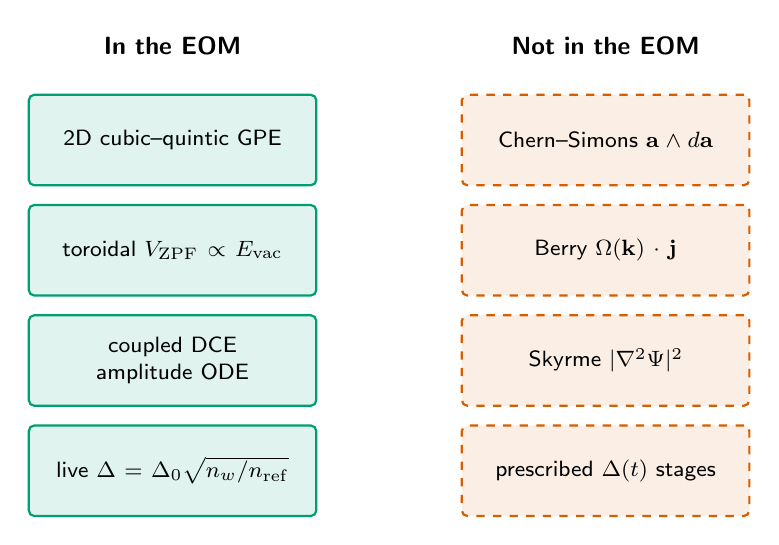
\begin{tikzpicture}[
  font=\sffamily\footnotesize,
  on/.style={draw=oiGreen, line width=0.8pt, fill=oiGreen!12, rounded corners=2pt,
    align=center, inner sep=5pt, text width=3.3cm, minimum height=1.15cm},
  off/.style={draw=oiVerm, line width=0.8pt, fill=oiVerm!10, rounded corners=2pt,
    align=center, inner sep=5pt, text width=3.3cm, minimum height=1.15cm, dashed},
]
\node[font=\sffamily\small\bfseries] (h1) at (0,3.35) {In the EOM};
\node[font=\sffamily\small\bfseries] (h2) at (5.5,3.35) {Not in the EOM};
\node[on] (a) at (0,2.15) {2D cubic--quintic GPE};
\node[on] (b) at (0,0.75) {toroidal $V_{\mathrm{ZPF}}\propto E_{\mathrm{vac}}$};
\node[on] (c) at (0,-0.65) {coupled DCE amplitude ODE};
\node[on] (d) at (0,-2.05) {live $\Delta=\Delta_0\sqrt{n_w/n_{\mathrm{ref}}}$};
\node[off] (e) at (5.5,2.15) {Chern--Simons $\mathbf{a}\wedge d\mathbf{a}$};
\node[off] (f) at (5.5,0.75) {Berry $\Omega(\mathbf{k})\cdot\mathbf{j}$};
\node[off] (g) at (5.5,-0.65) {Skyrme $|\nabla^2\Psi|^2$};
\node[off] (h) at (5.5,-2.05) {prescribed $\Delta(t)$ stages};
\end{tikzpicture}

\caption{Terms retained in the integrator (left) versus terms retained only in the parent functional or omitted as a prescribed gap schedule (right).}
\label{fig:trunc-s}
\end{figure}

The condensate field $\psi(x,y,t)$ obeys a cubic--quintic \GPE{} in two spatial dimensions,
\begin{equation}
i\hbar\partial_t\psi=\Bigl[-\frac{\hbar^2}{2m^*}\nabla^2+\alpha_0|\psi|^2+\beta|\psi|^4+V_{\mathrm{ZPF}}(\mathbf{r};A)+V_{\mathrm{ph}}(\mathbf{r},t)\Bigr]\psi,
\label{eq:gpe}
\end{equation}
with $\hbar=0.6582119569$\,meV$\cdot$ps in the integrator units. The vacuum potential is localized on the torus ring,
\begin{equation}
V_{\mathrm{ZPF}}(\mathbf{r};A)=-A\,E_{\mathrm{vac}}\exp\Bigl(-\frac{(\rho-R)^2}{2r^2}\Bigr),\qquad\rho=\sqrt{x^2+y^2},
\end{equation}
and $E_{\mathrm{vac}}$ is the working-cavity value $\Evac$. Explicitly, $V_{\mathrm{ZPF}}=-E_{\mathrm{vac}}(A(t)/A(0))$ times a ring Gaussian. The phonon drive on the $1$\,ps window is $V_{\mathrm{ph}}=0.1\Delta_0\sin(\omega_0 t)$ on the same ring, with $\omega_0=2\Delta_0/\hbar$.

The dynamical Casimir amplitude obeys the first-order law used in the integrator,
\begin{equation}
\dot A=\bigl[\Lambda(\Delta)\,\mathcal{L}(\delta\omega/\Gamma)-\Lambda_{\mathrm{loss}}\bigr]A,\qquad
\Lambda(\Delta)=\frac{m\Delta}{2\hbar}\frac{Q}{2\pi},\qquad
\mathcal{L}(x)=\frac{1}{1+x^2},
\label{eq:dce}
\end{equation}
with $\Lambda_{\mathrm{loss}}=\Gamma_{\mathrm{cav}}(\Delta^\star)$ the cavity linewidth, not a parameter fitted to $A^*/A_c=0.52$. Resonant driving uses $\omega_{\mathrm{pump}}/2=2\Delta^\star/\hbar$; the detuning-feedback run uses $\omega_{\mathrm{pump}}/2=2\Delta^\star/\hbar+2\Gamma$. On the coupled $1$\,ps window, $\Delta=\Delta_{\mathrm{live}}[\psi]$. On the $80$\,ps window, $\Delta$ is slaved to the physical fold branch $\Delta(A)$. The fold critical amplitude is $A_c^{\mathrm{fold}}=\Acfold$, not a BKT value.

Chern--Simons $\mathbf{a}\wedge d\mathbf{a}$, Berry $\Omega(\mathbf{k})\cdot\mathbf{j}$, and Skyrme $|\nabla^2\Psi|^2$ do \emph{not} appear in Eq.~\eqref{eq:gpe}. Any Hall staircase or hopfion charge quoted from dynamics is therefore an interpretation using the parent functional, not a flux measured on the grid.

\section{Live gap estimator}
\label{sec:live}

A previous solver stored
\begin{equation}
\Delta(t)\in\{0.600,0.389,0.200,0.032\}\,\mathrm{meV}
\end{equation}
as a function of time and did not use $\psi$. That function is not reimplemented.

Let $w(x,y)=\exp[-(\rho-R)^2/(2r^2)]$ be the ring weight. Define
\begin{equation}
n_w[\psi]=\frac{\sum_{ij} w_{ij}\,|\psi_{ij}|^2}{\sum_{ij} w_{ij}}.
\end{equation}
The primary estimator is
\begin{equation}
\Delta_{\mathrm{live}}[\psi]=\Delta_0\sqrt{\frac{n_w[\psi]}{n_{\mathrm{ref}}}},\qquad n_{\mathrm{ref}}=n_w[\psi(\,\cdot\,,0)].
\label{eq:dlive}
\end{equation}
Equation~\eqref{eq:dlive} has no time argument. If $n_w(0)=n_{\mathrm{ref}}$ then $\Delta_{\mathrm{live}}(0)=\Delta_0$. Secondary diagnostics are the density-weighted cubic--quintic potential $\langle\alpha_0|\psi|^2+\beta|\psi|^4\rangle_n$ and the first-order coherence
\begin{equation}
g^{(1)}=\frac{|\langle\psi\rangle|^2}{\langle|\psi|^2\rangle}.
\end{equation}
Coherence is a reportable output, not a license to omit Lindblad dissipation. The present truncation is Hamiltonian plus the DCE ODE; laboratory collapse would be weaker.

\section{Static comparison (fold, not a schedule)}
\label{sec:static}

Every dynamical run is compared to the locked fold, not to earlier inconsistent gap schedules. At working participation,
\begin{equation}
\lambda^\star=\lstar,\qquad\alpha^\star=0.90\,\alpha_c,\qquad\Delta^\star=\Deltastar
\end{equation}
on the physical branch. The integrator should be initialized near this static point (or near $\Delta_0$ with $\lambda$ ramped), never at $0.389$\,meV. The fold theorem forbids a static physical target of $0.032$\,meV: $\delta=0.032/0.6<\delta_c=\alphac$. Maximum static reduction is $\redmax$ at $\Delta_c=\Deltac$.

Drive-scale diagnostics that multiply historical rates by $E_{\mathrm{vac}}/0.244\approx 0.527$ are not split-step results and are not tabulated as physics.

\section{Initial data and grid}
\label{sec:grid}

The completed run uses a square box of side $200$\,nm, grid $128\times 128$, and $\mathrm{d}t=2$\,fs for a $1$\,ps coupled window. Kinetic coefficient $\hbar^2/(2m^*)=\Delta_0 a_H^2$ with $a_H=r=8$\,nm; cubic--quintic parameters $\alpha=-\Delta_0$, $\beta=\Delta_0/n_0$, $n_0=1$. The initial field is a hopfion with $10\%$ core depletion, phase $Q_H\theta$ with $Q_H=1/N=1/5$, and $3\%$ noise. The reference density $n_{\mathrm{ref}}$ is computed once from this field so that $\Delta_{\mathrm{live}}(0)=\Delta_0$. Time stepping is split-step Fourier for Eq.~\eqref{eq:gpe} and RK4 for Eq.~\eqref{eq:dce}. No output column named \texttt{delta\_prescribed} exists.

\section{Coupled GPE results ($1$\,ps)}
\label{sec:coupled}

\begin{table}[H]
\centering
\caption{Live-gap GPE window. All entries use $\psi$; none is a time schedule.}
\label{tab:gpe}
\begin{tabular}{@{}lc@{}}
\toprule
Quantity & Value \\
\midrule
$\Delta_{\mathrm{live}}(0)$ & $0.6000$\,meV \\
$\Delta_{\mathrm{live}}(1\,\mathrm{ps})$ & $\Deltaliveone$ \\
$\min\Delta_{\mathrm{live}}$ & $0.6000$\,meV \\
live ${}<{}\Delta_c$ & False \\
$g^{(1)}(1\,\mathrm{ps})$ & $\goneps$ \\
$A(1\,\mathrm{ps})/A_c^{\mathrm{fold}}$ & $\AoneAc$ \\
$\|\psi\|$ relative drift & $1.30\times 10^{-14}$ \\
\bottomrule
\end{tabular}
\end{table}

The live gap \emph{increases}. That is the result. It is not a $92\%$ collapse, and it is not spun as a delayed catalyzation: the truncated Hamiltonian plus a $1$\,ps drive simply did not deplete the ring-weighted density below $n_{\mathrm{ref}}$.

\begin{figure}[H]
\centering
% Coupled GPE 1 ps: live gap from psi (not a schedule)
\begin{tikzpicture}
\begin{axis}[
  width=0.92\linewidth,
  height=5.6cm,
  xlabel={$t$ (ps)},
  ylabel={$\Delta_{\mathrm{live}}[\psi]$ (meV)},
  xmin=0, xmax=1.02,
  ymin=0.08, ymax=0.72,
  legend style={draw=none, at={(0.02,0.98)}, anchor=north west, font=\footnotesize},
  tick label style={font=\small},
  label style={font=\small},
]
\addplot[oiBlue, thick]
  table[col sep=comma, x=t_ps, y=Delta_live_meV] {data/coupled_timeseries_plot.csv};
\addlegendentry{$\Delta_{\mathrm{live}}$}
\addplot[oiOrange, densely dashed]
  table[col sep=comma, x=t_ps, y=Delta_fold_of_A_meV] {data/coupled_timeseries_plot.csv};
\addlegendentry{fold $\Delta(A)$}
\addplot[oiGreen, densely dotted] coordinates {(0,0.600) (1.02,0.600)};
\addlegendentry{$\Delta_0$}
\addplot[oiVerm, densely dotted] coordinates {(0,0.1091) (1.02,0.1091)};
\addlegendentry{$\Delta_c$}
\end{axis}
\end{tikzpicture}

\caption{Live gap versus the instantaneous fold branch $\Delta(A)$ on the $1$\,ps window. Guides: $\Delta_0$ and $\Delta_c$.}
\label{fig:live-s}
\end{figure}

\begin{figure}[H]
\centering
% Coupled GPE: coherence and DCE amplitude
\begin{tikzpicture}
\begin{axis}[
  width=0.92\linewidth,
  height=5.4cm,
  xlabel={$t$ (ps)},
  ylabel={$g^{(1)}$,\ $A/A_c^{\mathrm{fold}}$},
  xmin=0, xmax=1.02,
  ymin=0.82, ymax=1.02,
  legend style={draw=none, at={(0.02,0.02)}, anchor=south west, font=\footnotesize},
  tick label style={font=\small},
  label style={font=\small},
]
\addplot[oiPurple, thick]
  table[col sep=comma, x=t_ps, y=g1] {data/coupled_timeseries_plot.csv};
\addlegendentry{$g^{(1)}$}
\addplot[oiBlue, thick, dashed]
  table[col sep=comma, x=t_ps, y expr={\thisrow{A_um_inv}/1.558248}] {data/coupled_timeseries_plot.csv};
\addlegendentry{$A/A_c^{\mathrm{fold}}$}
\end{axis}
\end{tikzpicture}

\caption{Coherence $g^{(1)}$ and $A/A_c^{\mathrm{fold}}$ on the same window.}
\label{fig:g1-s}
\end{figure}

\section{Fold-slaved DCE ($80$\,ps)}
\label{sec:dcerun}

\begin{table}[H]
\centering
\caption{DCE saturation. Ratios are computed from $A_c^{\mathrm{fold}}=\Acfold$; $0.52$ is not imposed.}
\label{tab:dce}
\begin{tabular}{@{}lccc@{}}
\toprule
Case & $A^*/A_c^{\mathrm{fold}}$ & $\Delta_{\mathrm{ss}}$ (meV) & $L(0)$ \\
\midrule
resonant & $\AresAc$ & $0.2240$ & $1.000$ \\
detuning & $\AdetAc$ & $0.2461$ & $0.200$ \\
\bottomrule
\end{tabular}
\end{table}

Neither run folded out. Two-timescale justification: $\Gamma_{\mathrm{cav}}^{-1}$ is tens of picoseconds, much longer than the $1$\,ps GPE window, so the $80$\,ps amplitude uses $\Delta$ slaved to the physical fold branch rather than a live $\psi$.

\begin{figure}[H]
\centering
% Fold-slaved DCE, 80 ps (A*/A_c computed, not 0.52)
\begin{tikzpicture}
\begin{axis}[
  width=0.92\linewidth,
  height=5.6cm,
  xlabel={$t$ (ps)},
  ylabel={$A(t)/A_c^{\mathrm{fold}}$},
  xmin=0, xmax=80,
  ymin=0.82, ymax=0.96,
  legend style={draw=none, at={(0.98,0.02)}, anchor=south east, font=\footnotesize},
  tick label style={font=\small},
  label style={font=\small},
]
\addplot[oiBlue, thick]
  table[col sep=comma, x=t_ps, y expr={\thisrow{A_um_inv}/1.558248}] {data/dce_resonant_plot.csv};
\addlegendentry{resonant $L(0)=1$}
\addplot[oiOrange, thick, dashed]
  table[col sep=comma, x=t_ps, y expr={\thisrow{A_um_inv}/1.558248}] {data/dce_detuning_plot.csv};
\addlegendentry{detuned $L(0)=0.2$}
\end{axis}
\end{tikzpicture}

\caption{Fold-slaved DCE amplitude in units of $A_c^{\mathrm{fold}}$. Resonant (solid) and detuned (dashed) saturations are $\AresAc$ and $\AdetAc$.}
\label{fig:dce-s}
\end{figure}

\begin{figure}[H]
\centering
% DCE Lorentzian (fold-slaved)
\begin{tikzpicture}
\begin{axis}[
  width=0.92\linewidth,
  height=5.2cm,
  xlabel={$t$ (ps)},
  ylabel={Lorentzian $\mathcal{L}$},
  xmin=0, xmax=80,
  ymin=0, ymax=1.05,
  legend style={draw=none, at={(0.98,0.98)}, anchor=north east, font=\footnotesize},
  tick label style={font=\small},
  label style={font=\small},
]
\addplot[oiBlue, thick]
  table[col sep=comma, x=t_ps, y=lorentzian] {data/dce_resonant_plot.csv};
\addlegendentry{resonant}
\addplot[oiOrange, thick, dashed]
  table[col sep=comma, x=t_ps, y=lorentzian] {data/dce_detuning_plot.csv};
\addlegendentry{detuned}
\end{axis}
\end{tikzpicture}

\caption{Lorentzian $\mathcal{L}(\delta\omega/\Gamma)$ on the same $80$\,ps runs.}
\label{fig:lor-s}
\end{figure}

\section{Coupling matrix $G_{ij}$}
\label{sec:gij}

\subsection{Democratic lock}

For $G=g_0(J_N-I_N)$ the spectrum is exact:
\begin{equation}
\lambda_{\max}=(N-1)g_0\quad(\mathrm{mult.\ }1),\qquad
\lambda_{\min}=-g_0\quad(\mathrm{mult.\ }N-1).
\end{equation}
Helmert (sum-zero) vectors span the dark subspace. The catalyzon shift is $\Delta_{\mathrm{cat}}=\Delta_{\mathrm{ex}}-g_0$. A previously used working value $g_0=0.21$\,meV is larger than $E_{\mathrm{vac}}$ and is not a vacuum scale. The identification used in Schwinger/Berry diagnostics is $g_0=\lambda^\star E_{\mathrm{vac}}=\gzerostar$, so $|\lambda_{\min}|=\gzerostar$. The older scaling $g_0\approx\gzeroscaled$ ($\lambda_{\mathrm{cat}}\approx\lamcat$) remains a distinct guess from $0.1\times E_{\mathrm{vac}}/0.244$ and is not mixed with $\gzerostar$.

\begin{figure}[H]
\centering
% Democratic Spec(G)
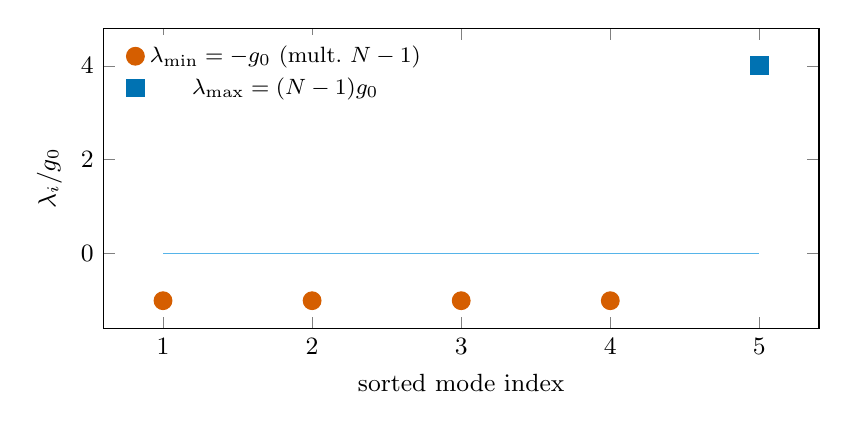
\begin{tikzpicture}
\begin{axis}[
  width=0.88\linewidth,
  height=5.4cm,
  xlabel={sorted mode index},
  ylabel={$\lambda_i/g_0$},
  xtick={1,2,3,4,5},
  ymin=-1.6, ymax=4.8,
  legend style={draw=none, at={(0.02,0.98)}, anchor=north west, font=\footnotesize},
  tick label style={font=\small},
  label style={font=\small},
]
\addplot[only marks, mark=*, mark size=3.2pt, oiVerm]
  coordinates {(1,-1)(2,-1)(3,-1)(4,-1)};
\addlegendentry{$\lambda_{\min}=-g_0$ (mult.\ $N-1$)}
\addplot[only marks, mark=square*, mark size=3.2pt, oiBlue]
  coordinates {(5,4)};
\addlegendentry{$\lambda_{\max}=(N-1)g_0$}
\addplot[oiSky, thin] coordinates {(1,0)(5,0)};
\end{axis}
\end{tikzpicture}

\caption{Democratic spectrum used as the algebraic lock. WS numerics are compared to this figure, not to $\lambda_{\min}=-4g_0$.}
\label{fig:spec-s}
\end{figure}

\subsection{Wigner--Seitz overlap computation}

Five Gaussians of width $\sigma\approx 0.18\,\lambda_M$ are placed at the vertices of a regular pentagon inscribed in the moir\'e hexagon of period $\lambda_M=13$\,nm. Off-diagonal entries are overlaps against $K_0(|\mathbf{r}-\mathbf{r}'|/\xi_K)$ with $\xi_K=R=50$\,nm; the diagonal is set to zero. Democratic $J-I$ is not inserted. Reported acceptance tests are: Hermitian, $G_{ii}=0$, $\operatorname{Tr} G=0$, $\lambda_{\min}<0$, and relative Frobenius distance $\approx 7.0\%$ to the democratic matrix at $\langle G_{\mathrm{off}}\rangle$. Dark multiplicity is split, as expected for a pentagon in a hexagon. Eigenvalues remain $\mathcal{O}(10^{-4})$ in kernel units; converting to meV requires the missing prefactor $\kappa$ such that $g_0=\lambda_G E_{\mathrm{vac}}$.

Heatmaps of this overlap are archived with the paper figures. They document a computed kernel, not a torsion variation of $S_{\mathrm{FN}}+S_{\mathrm{sf}}+S_{\mathrm{int}}$.

\subsection{Cartan-torsion origin of \texorpdfstring{$G_{ij}$}{Gij} is not evaluated}

The conjectured vertex
\begin{equation}
G_{ij}\stackrel{?}{=}\frac{\kappa_{\mathrm{tor}}}{4\pi^2}\int_{\mathrm{WS}}\varepsilon^{\mu}{}_{\nu\rho\sigma}\,
\partial_\sigma q_H\,\Phi_i^{*\nu}\Phi_j^\rho\,\mathrm{d}^3x
\end{equation}
is not evaluated. Passing Wigner--Seitz acceptance tests does not establish a torsion origin. The two-dimensional proxy of the main-text closure is not democratic; a 3D Weitzenb\"ock quadrature is left for future work and is not used to set $G_{ij}$ or $g_0^\star$.

\section{Parallel channels (do not stack)}
\label{sec:parallel}

\begin{figure}[H]
\centering
% Parallel channels
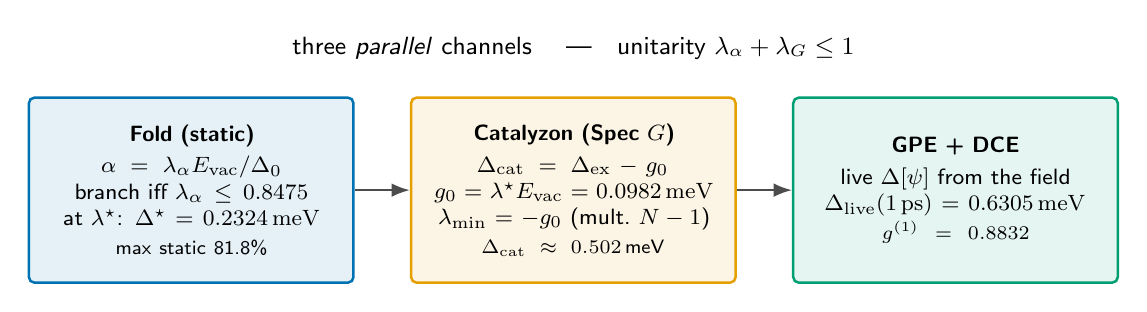
\begin{tikzpicture}[
  font=\sffamily\footnotesize,
  ch/.style={draw=#1, line width=0.9pt, rounded corners=2pt, fill=#1!10,
    align=center, inner sep=6pt, text width=3.7cm, minimum height=2.35cm},
  arr/.style={-{Latex}, thick, gray!60!black}
]
\node[ch=oiBlue] (f) {\textbf{Fold (static)}\\[2pt]
$\alpha=\lambda_\alpha E_{\mathrm{vac}}/\Delta_0$\\
branch iff $\lambda_\alpha\le\lfold$\\
at $\lambda^\star$: $\Delta^\star=\Deltastar$\\[1pt]
{\scriptsize max static \redmax}};
\node[ch=oiOrange, right=0.7cm of f] (c) {\textbf{Catalyzon (Spec $G$)}\\[2pt]
$\Delta_{\mathrm{cat}}=\Delta_{\mathrm{ex}}-g_0$\\
$g_0=\lambda^\star E_{\mathrm{vac}}=\gzerostar$\\
$\lambda_{\min}=-g_0$ (mult.\ $N-1$)\\[1pt]
{\scriptsize $\Delta_{\mathrm{cat}}\approx 0.502$\,meV}};
\node[ch=oiGreen, right=0.7cm of c] (t) {\textbf{GPE + DCE}\\[2pt]
live $\Delta[\psi]$ from the field\\
$\Delta_{\mathrm{live}}(1\,\mathrm{ps})=\Deltaliveone$\\[1pt]
{\scriptsize $g^{(1)}=\goneps$}};
\node[above=0.35cm of c, font=\sffamily\small, align=center]
  {three \emph{parallel} channels \quad---\quad unitarity $\lambda_\alpha+\lambda_G\le 1$};
\draw[arr] (f.east) -- (c.west);
\draw[arr] (c.east) -- (t.west);
\end{tikzpicture}

\caption{Fold, catalyzon, and GPE/DCE are parallel. Earlier stacked percentages mixed distinct baselines and a prescribed $\Delta(t)$.}
\label{fig:ch-s}
\end{figure}

The completed $1$\,ps run has $\Delta_{\mathrm{live}}(1\,\mathrm{ps})=\Deltaliveone>\Delta_c$, so it is not an overshoot of the fold. A future run that did fall below $\Delta_c$ would be flagged unphysical versus the static branch and would still not resurrect $0.032$\,meV.

\section{Schwinger and Berry (not in the EOM)}
\label{sec:schberry}

With $g_0=\lambda^\star E_{\mathrm{vac}}=\gzerostar$ one has $E_{\mathrm{pair}}=2|\lambda_{\min}|=\Epair$. The diagnostic crossover is $T^*=\Tstar$. The GOE/GUE Monte Carlo ratio of mean $|\lambda_{\min}|$ is $R_{\mathrm{mean}}=\BerryR$, not a forced $1.43$ enhancement. These numbers are not terms in Eq.~\eqref{eq:gpe}.

\section{Earlier dynamical claims not used here}
\label{sec:withdrawn}

The v3 ``three-stage collapse'' identified (i)~bare $\to$ self-consistent $0.600\to 0.389$\,meV as a $35\%$ static loop at $E_{\mathrm{Cas}}=0.244$\,meV; (ii)~a $52\%$ catalyzon mix $(\Delta_{\mathrm{QVC}}-0.1)/\Delta_{\mathrm{ex}}$; (iii)~a coherent $92\%$ drop $(0.389-0.032)/0.389$ over $1$\,ps with $V_{\mathrm{ZPF}}=-0.244$\,meV. Stage~(i) is fold-out under the derived bridge. Stage~(ii) is not $\mathrm{Spec}(G)$ at $g_0=\gzerostar$. Stage~(iii) used a gap function of time, not of $\psi$, and landed below $\delta_c$. The live-gap calculation instead gives $\Deltaliveone$ at $1$\,ps.

\section{Reading of the completed run}
\label{sec:readout}

Figures~\ref{fig:live-s}--\ref{fig:lor-s} report $\Delta_{\mathrm{live}}(t)$, $g^{(1)}(t)$, and $A(t)$ with guides at $\Delta_0$ and $\Delta_c$. Because $\Delta_{\mathrm{live}}$ rose while $g^{(1)}$ stayed of order one, the $1$\,ps window is a coherent non-collapse of the truncated GPE, not catalyzation through the fold and not dephasing. Hall conductance is not an output of Eq.~\eqref{eq:gpe}; it remains a prediction of $Q_H=1/N$ awaiting a Chern--Simons integrator.

\section{Reproducibility}
\label{sec:repro}

Fold and vacuum numbers are regenerated from the source accompanying the preprint at \url{https://github.com/mineralhoiland/QVC}. Time series for the live-gap and dynamical Casimir runs are stored with the paper data files. Compilation of this PDF does not re-execute the Gross--Pitaevskii integrator.

\bibliographystyle{unsrt}
\bibliography{qvc_refs}

\end{document}
